\label{chpt:results:three peculiar white dwarfs} % for referencing this chapter elsewhere, use \ref{chpt:label}
\lhead{\emph{Three CVs with peculiar white dwarf colours}} % This is for the header on each page - perhaps a shortened title


The work presented in this chapter was published as \cite{wild2021}, in the Monthly Notices of the Royal Astronomical Society under the title \textit{System parameters of three short period cataclysmic variable stars} by Wild, Littlefair, Ashley, Breedt, Brown, Dhillon, Dyer, Green, Kerry, Marsh, Parsons, and Sahman.
The following is my own work, unless otherwise cited.

This chapter concerns the three systems, ASASSN-16kr, ASASSN-17jf, and CRTS SSSJ0522-3505 J052210-350530 (hereafter SSSJ0522-3505), which proved challenging to model.
Phase-folded eclipse modelling gave good results in all three systems, each lightcurve being well-modelled with small residuals.
The Gaussian processes describing flickering in the systems were consistent with little to no variability, indicating that almost all the scatter in the flux residuals could be fully described by the uncertainty in flux measurement.
For a catalogue of the fits, see Appendix~\ref{appendix:lightcurves}, though an example eclipse from the ASASSN-16kr observations is shown here in Figure~\ref{fig:three white dwarfs:ASASSN-16kr example lightcurves}.
However, when fitting white dwarf model atmospheres to the observed white dwarf fluxes, the resulting fits were not satisfactory. The bulk of this chapter discusses this poor fit, and explores its implications.

% Also included is a rudimentary attempt to examine the modern understanding of CV evolution, using the excess period as a rough diagnostic of excess AML. The implications of this early method is compared to the newer, more quantitative method described in \S\ref{sect:modelling:evolutionary modelling}.

\begin{figure*}
    \centering
    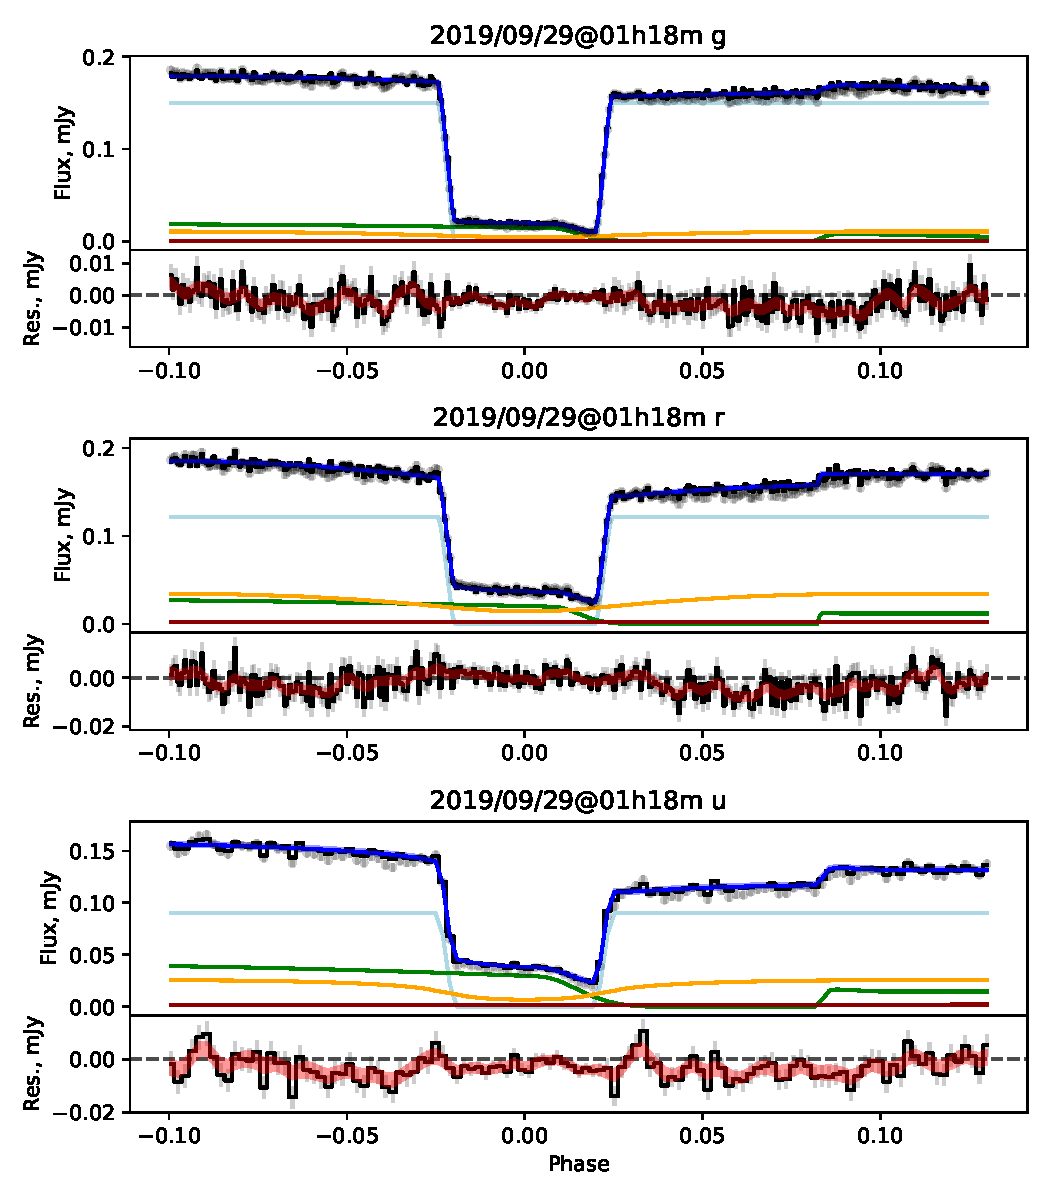
\includegraphics[width=\textwidth]{figures/results/three_cvs_with_weird_colours/ASASSN-16kr/ASASSN-16kr_sample.pdf}
    \caption{ASASSN-16kr example lightcurve models. {\it Top}:~{\bf grey points} are the observed flux; {\bf black line} is the observed flux, with the mean Gaussian process sample subtracted; the {\bf dark blue line} is the mean lightcurve model, and the {\bf blue band} is the standard deviation on this in the MCMC chain. The components of the model are also shown: the {\bf light blue line} is the white dwarf flux, {\bf green line} is the bright spot, {\bf orange line} is the disc, and the {\bf red line} is the donor. {\it Bottom}:~The residuals between the data and model are plotted as the {\bf black line with grey error bars}. The Gaussian process 1-sigma region is shown as a {\bf red band}. A catalogue of all such fits in this work is given in Appendix~\ref{appendix:lightcurves}.}
    \label{fig:three white dwarfs:ASASSN-16kr example lightcurves}
\end{figure*}


\section{White dwarf atmosphere fits}
\label{sect:three white dwarfs:method WD atmosphere fits}

The two values of $\log (g)$ produced by modelling -- the first from fitting the white dwarf fluxes to model atmospheres, and the second from combining $T_{\rm eff}$ and $P$ with the lightcurve parameters -- did not fall within $1\sigma$ of each other in any of these three systems.
In ASASSN-17jf and SSSJ0522-3505, the white dwarf atmosphere fit converged close to the minimum surface gravity allowed by the coverage of our models, $\log(g) = 7.0$.
The second $\log (g)$, from lightcurve fitting, indicated values for each system of $8.10\pm0.04$ and $8.30\pm0.03$, respectively.
When analysing ASASSN-16kr, flux fitting gave a more reasonable $\log(g)=8.21\pm0.13$, but the second $\log (g)$ still gave a significantly higher $\log(g)=8.59\pm0.03$, a difference of $\sim3\sigma$.

This is concerning, as the two $\log (g)$\ should be consistent with one another for each system.
Comparison of the measured white dwarf colours to the \citet{Bergeron1995} model grids in Figures \ref{fig:ASASSN-17jf colours}, \ref{fig:ASASSN-16kr colours}, and \ref{fig:SSSJ0522-3505 colours}, reveals that the measured colours of the white dwarfs lie outside the colour space of the models. This is the origin of the discrepancies in $\log (g)$\ obtained with the two methods for ASASSN-17jf and SSSJ0522-3505, but ASASSN-16kr is consistent with the rightmost cooling track. However, the observed flux of a white dwarf of this radius is too high for the observed Gaia parallax, pushing the model fits to smaller, higher gravity model atmospheres.

A likely cause for this issue would be an error in photometric calibration, causing a corresponding error in white dwarf fluxes. However, this is unlikely to be the source of the problem, for the reasons explained in \S\ref{sect:observations:flux calibrating the lightcurve}.
Inspection of the figures in Appendix~\ref{appendix:lightcurves} also rules out poor lightcurve fits as the cause of this problem. The most plausible explanation for the fact that our measured white dwarf fluxes do not lie inside the model grids, is that the change in brightness during white dwarf ingress/egress is contaminated by an additional source of light, for example a boundary layer close to the white dwarf surface. The implications of this for our system parameters is explored in \S\ref{sect:impure white dwarf discussion}.

That the white dwarf colours do not lie on the model grids also raises questions about the accuracy of the white dwarf temperatures. To try and quantify the impact on $T_{\rm eff}$, two additional optimisations of model parameters to the white dwarf fluxes were performed.
In one approach, a Gaussian prior on $\log (g)$\ using the estimate from the lightcurve modelling was used, and all available flux measurements were fit simultaneously.
In a second approach we fit the white dwarf flux in each band independently using the same prior on $\log (g)$\ and the Gaia prior on $\pi$. Since these independent fits use no colour information, E(B-V) is only constrained by the prior, but is retained as a nuisance parameter and $T_{\rm eff}$ is marginalised over E(B-V). Figure~\ref{fig:three white dwarfs:gamma fits} shows the $T_{\rm eff}$ posteriors from the individual fits for the three systems.

\begin{figure}
    \centering
    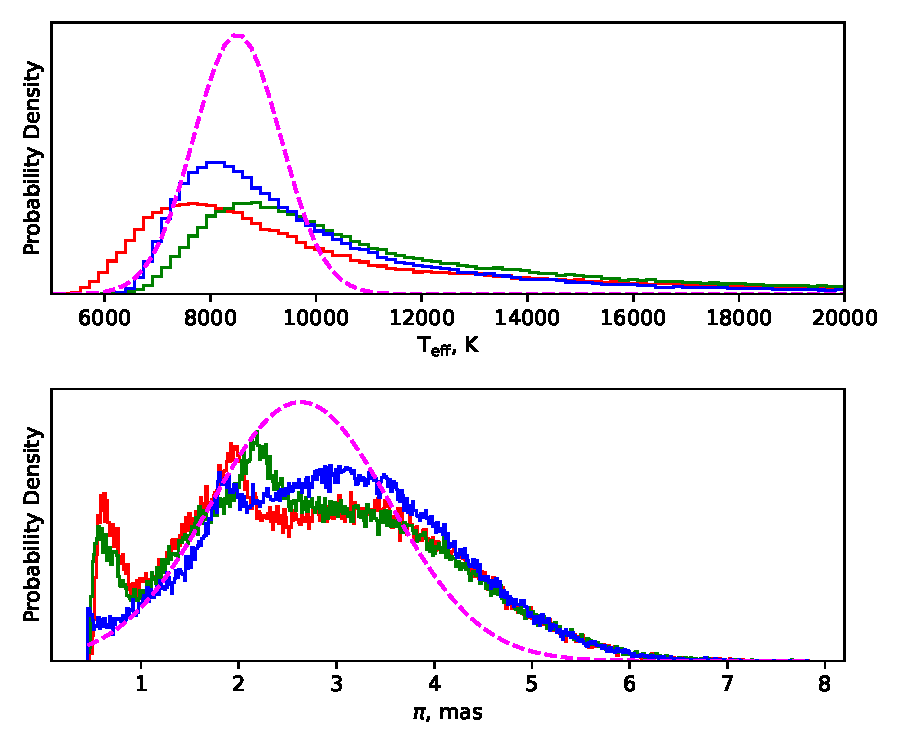
\includegraphics[width=\columnwidth, trim={0cm 6.5cm 0cm 0cm}, clip]{figures/results/three_cvs_with_weird_colours/ASASSN-17jf/PhysicalParams/all_gamma_asassn17jf.pdf}
    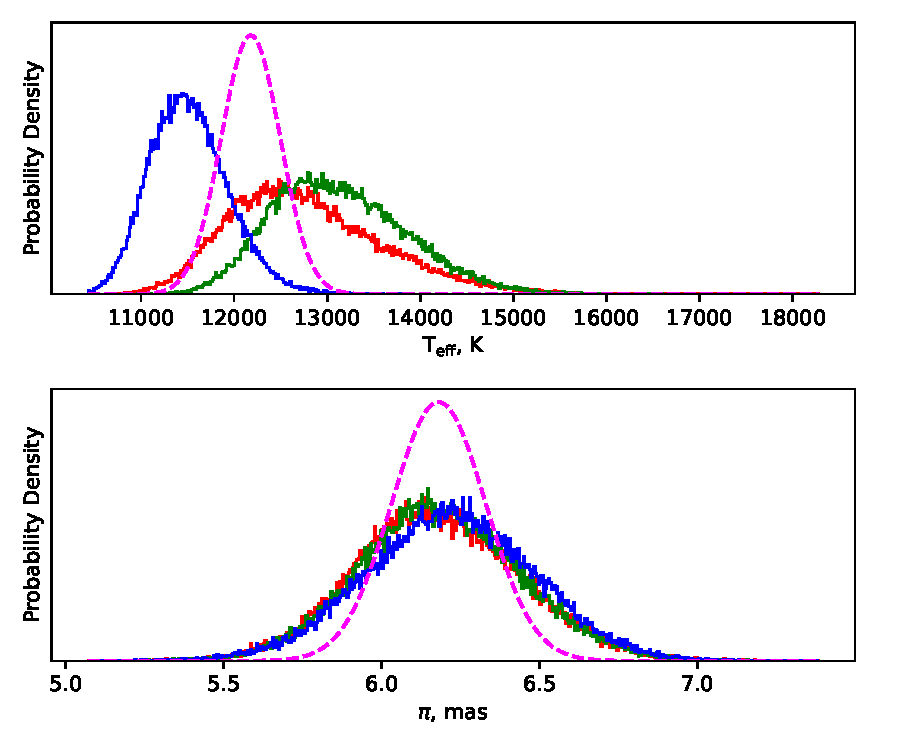
\includegraphics[width=\columnwidth, trim={0cm 6.5cm 0cm 0cm}, clip]{figures/results/three_cvs_with_weird_colours/ASASSN-16kr/PhysicalParams/all_gamma_asassn16kr.pdf}
    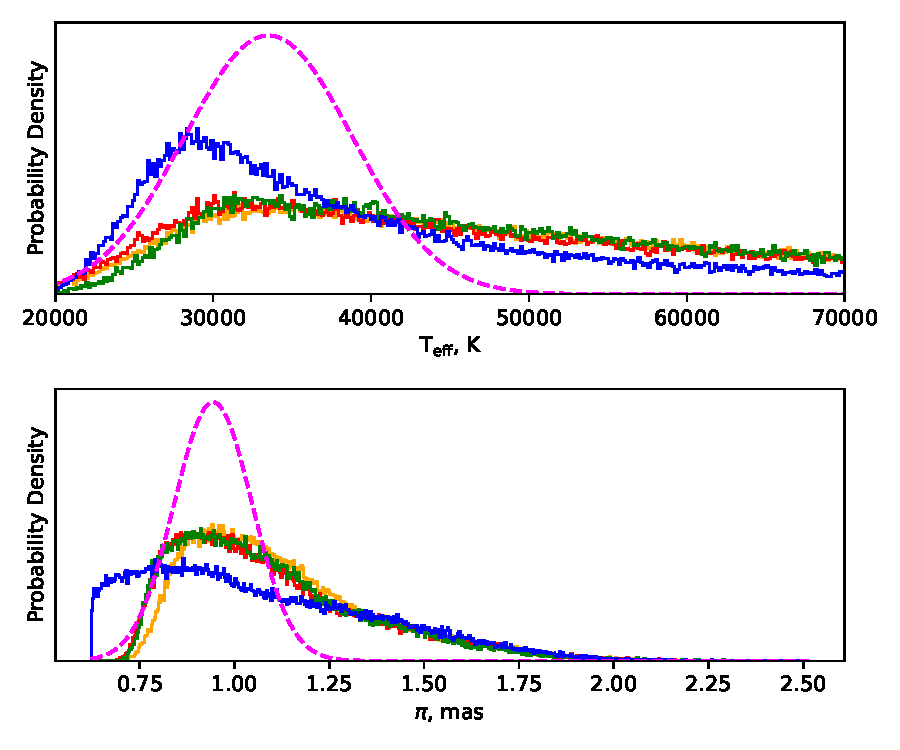
\includegraphics[width=\columnwidth, trim={0cm 6.5cm 0cm 0cm}, clip]{figures/results/three_cvs_with_weird_colours/SSS111126/PhysicalParams/all_gamma_SSS111126.pdf}
    \caption{The result of fitting white dwarf model atmospheres to each photometric band independently. {\bf Blue solid line}: $u'$ band, {\bf Green solid line}: $g'$ band, {\bf Red solid line}: $r'$ band. The joint distribution between all bands is characterised in each case by the best fit Gaussian ({\bf magenta dashed lines}). \textit{Top}: ASASSN-17jf, joint $T_{\rm eff}=8330\pm780\rm\ K$; \textit{Middle}: ASASSN-16kr, joint $T_{\rm eff}=12150\pm300\rm\ K$; \textit{Bottom}: SSSJ0522-3505, joint $T_{\rm eff}=33300\pm5200 \rm\ K$. }
    \label{fig:three white dwarfs:gamma fits}
\end{figure}

Figure \ref{fig:three white dwarfs:gamma fits} shows little sign of a consistent discrepancy over the three observed CVs. The $u'$ band in ASASSN-16kr and SSSJ0522-3505 suggests a cooler temperature than the other bands, but lies in between the $r'$ and $g'$ in ASASSN-17jf.


% \subsection{White dwarf temperature fits}
% \label{sect:white dwarf temperature report}

Each approach gives a different distribution for $T_{\rm eff}$.
To avoid confusion, results of each individual fit are not reported, instead the overall temperature ranges for each system are given.
ASASSN-16kr $T_{\rm eff}$ estimates ranged from 10200K to 12150K, and ASASSN-17jf estimates from 8330K to 12710K.
The SSSJ0522-3505 fits that used all four observed fluxes both converged on $\sim22700$K, but the single-flux fits all resulted in wide posterior distributions covering $25000 - 90000$K, with very weak peaks in the $\sim30000 - 50000$K range, seen in Figure~\ref{fig:three white dwarfs:gamma fits}.

In all three systems, the figures reported in Table~\ref{table:three white dwarfs:system_parameters main} are the $T_{\rm eff}$ produced by the constrained $\log (g)$ fit with all fluxes simultaneously.
The $\log (g)$ reported are the values found from the lightcurve parameters.


\section{System Parameters}
\label{sect:system parameters}

The effect of the uncertain white dwarf temperatures on the system parameters, most importantly $M_{\rm wd}$, is mostly negligible. For example, increasing $T_{\rm eff}$ for ASASSN-17jf from 8000K to 12000K only changes $M_{\rm WD}$ by $0.001M_\odot$, compared to our statistical uncertainty of $0.031 M_\odot$. Even a large uncertainty in $T_{\rm eff}$ only has a minor impact on the system parameters; for example a change in the WD temp for SSSJ0522-3505 from $10000$K to $20000$K only changes $M_{\rm WD}$ by $0.02 M_\odot$, comparable with the measurement uncertainty. The system parameters are reported in Table~\ref{table:three white dwarfs:system_parameters main}.

ASASSN-16kr has a recorded superhump period, and now also a $q$ measurement. It can therefore be used to calibrate the superhump period excess, $\epsilon$ vs. $q$ relationship, as done in \citet{McAllister2019}, though with a more extreme mass ratio system than was previously available. The system was not confidently classed as exhibiting stage B or C stage superhumps, so the results for both stages are given. Assuming the CV was in stage B, $q_B = 0.059\pm0.007$; assuming stage C and using the relevant relation from \citet{McAllister2019}, $q_C = 0.068\pm0.012$. In both cases, the estimated $q_\mathrm{B,C}$ is $\sim 2 \sigma$ higher than the observed value of $q = 0.044\pm0.002$. While a $2 \sigma$ difference is not a highly significant discrepancy, this may be preliminary evidence that the $\epsilon - q$ relation may over estimate $q$ for CVs at short periods, which has been suspected for some time \citep{pearson2007, knigge11}.

\begin{figure}
    \centering
    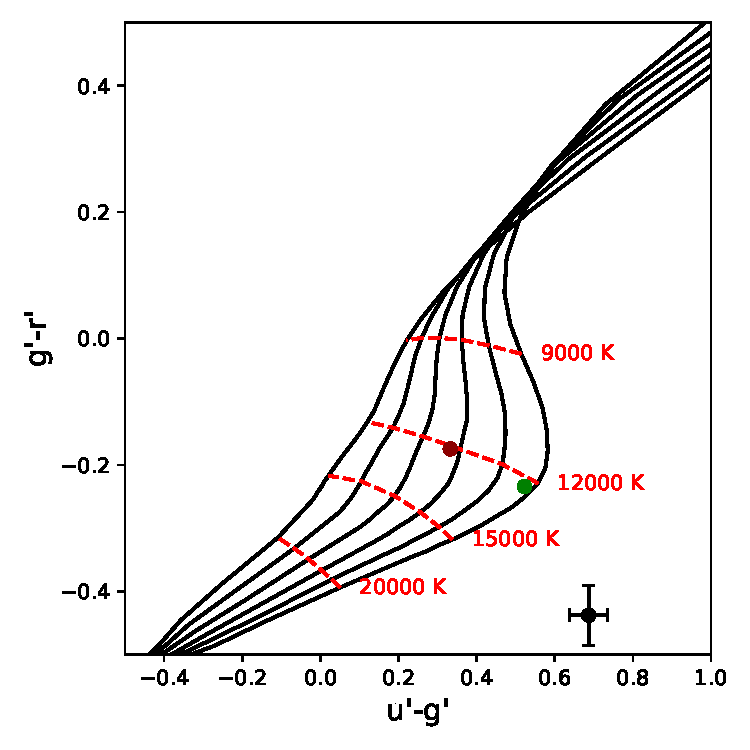
\includegraphics[width=\columnwidth, trim={0 0mm 0 0},clip]{figures/results/three_cvs_with_weird_colours/ASASSN-17jf/PhysicalParams/ASASSN-17jf_colourPlot_alpha_beta.pdf}
    \caption{The white dwarf model atmosphere fits for ASASSN-17jf. {\bf Green circle}: Best fit with uniform prior on $\log (g)$. {\bf Red circle}: Best fit with the prior $\log(g)=8.10\pm0.04$. The observations are shown as the {\bf black point and error bars}. {\bf Solid black lines} are white dwarf model cooling tracks, increasing in $\log (g)$\ to the left. {\bf Red dashed lines} are isothermal tracks for different $\log (g)$.}
    \label{fig:ASASSN-17jf colours}
\end{figure}
\begin{figure}
    \centering
    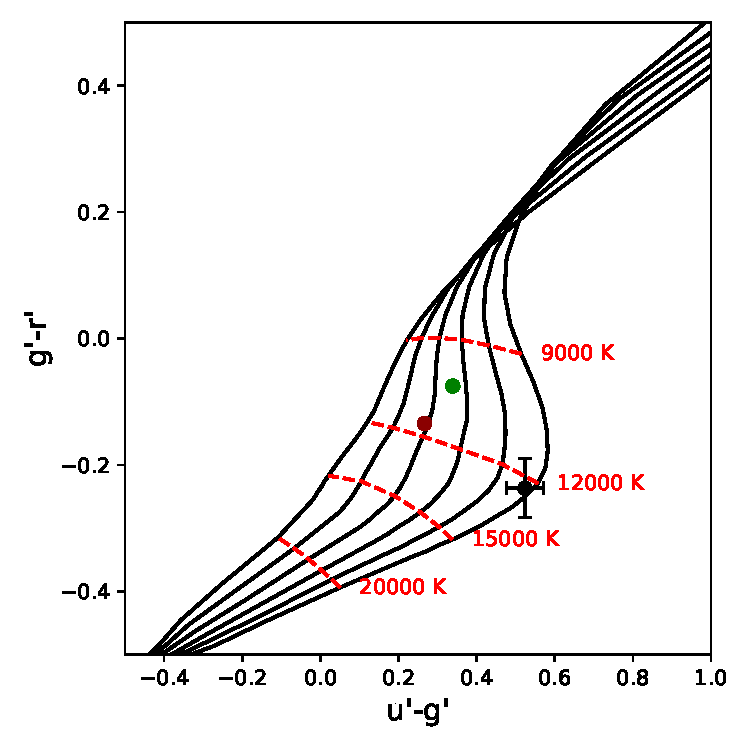
\includegraphics[width=\columnwidth, trim={0 0mm 0 0},clip]{figures/results/three_cvs_with_weird_colours/ASASSN-16kr/PhysicalParams/ASASSN-16kr_colourPlot_alpha_beta.pdf}
    \caption{The white dwarf model atmosphere fits for ASASSN-16kr. The {\bf red circle} is the best fit with a prior of $\log(g)=8.52\pm0.02$. Symbols are the same as Figure~\ref{fig:ASASSN-17jf colours}.}
    \label{fig:ASASSN-16kr colours}
\end{figure}
\begin{figure}
    \centering
    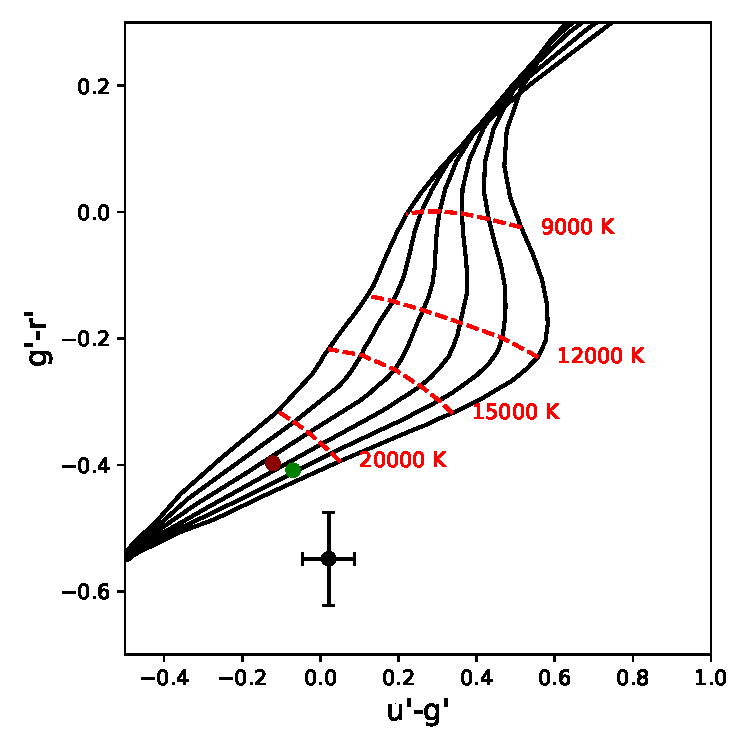
\includegraphics[width=\columnwidth, trim={0 0 0 0}, clip]{figures/results/three_cvs_with_weird_colours/SSS111126/PhysicalParams/SSS111126_colourPlot_alpha_beta.pdf}
    \caption{The white dwarf model atmosphere fits for SSSJ0522-3505. The {\bf red circle} is the best fit with a prior of $\log(g)=8.28\pm0.04$. Symbols are the same as Figure~\ref{fig:ASASSN-17jf colours}.}
    \label{fig:SSSJ0522-3505 colours}
\end{figure}

\begin{table*}
    \centering
    \caption{The system parameters found for the three CVs with peculiar white dwarf colours. Here, the reported $\pi$ is the posterior distribution from fitting the white dwarf fluxes, c.f. \S\ref{sect:modelling:fitting white dwarf colours}.}
    \label{table:three white dwarfs:system_parameters main}
    \begin{tabular}{cccc}
        \hline \\
        \textbf{System Name:}      & \textbf{ASASSN-16kr}    & \textbf{ASASSN-17jf}  & \textbf{SSSJ0522-3505} \\
        \hline \hline \\
        $M_\mathrm{WD}/M_\odot$    & $0.952\pm0.018$         & $0.669\pm0.031$        & $0.760\pm0.023$ \\
        $R_\mathrm{WD}/R_\odot$    & $0.0083\pm0.0002$       & $0.0120\pm0.0004$      & $0.0112\pm0.0003$ \\
        $M_\mathrm{donor}/M_\odot$ & $0.042\pm0.001$         & $0.060\pm0.008$        & $0.042\pm0.004$ \\
        $R_\mathrm{donor}/R_\odot$ & $0.105\pm0.002$         & $0.112\pm0.004$        & $0.105\pm0.004$ \\
        $q$                        & $0.044\pm0.002$         & $0.085\pm0.006$        & $0.055\pm0.003$ \\
        \hline
        $P$, hours                 & $1.470862368(2)$        & $1.36297(2)$           & $1.492642(2)$ \\
        $a/R_\odot$,               & $0.653\pm0.005$         & $0.567\pm0.009$        & $0.614\pm0.007$  \\
        $i$                        & $86.4\pm0.4$            & $83.7\pm0.5$           & $83.8\pm0.3$  \\
        $K_\mathrm{WD}$, km/s      & $22.7\pm1.5$            & $39.5\pm4.2$           & $26.0\pm1.8$  \\
        $K_\mathrm{donor}$, km/s   & $515\pm3$               & $462\pm5$              & $470\pm4$  \\
        \hline
        $\pi$, mas                 & $6.58\pm0.22$           & $2.09\pm0.19$          & $1.81\pm0.11$  \\
        $T_{\rm eff}$, kK          & $10-12$                 & $8-13$                 & $\sim25$  \\
        $\log(g), {\rm cgs}$       & $8.55\pm0.03$           & $8.15\pm0.05$          & $8.22\pm0.04$  \\
        \hline
    \end{tabular}
\end{table*}


\section{Implications of results}
\label{sect:discussion:three CVs with peculiar white dwarf colours}

All three systems were candidate post-period minimum systems based on their periods and preliminary eclipse data; none show a prominent bright spot (indicative of a low mass transfer rate), or significant donor flux (implying a dim donor).
As a result of this work, ASASSN-16kr and SSSJ0522-3505 are confirmed as having evolved through the period minimum and now have sub-stellar donors, and ASASSN-17jf lies in the period minimum region of Figure~\ref{fig:M2_vs_P}.
Additionally, all three white dwarf masses derived in this analysis fall within the range of CV white dwarf masses observed by \citet{pala2020}, of $\langle M_{\rm WD}\rangle = 0.83 \pm 0.17 M_\odot$, significantly higher than the pre-CV DA white dwarf mass of only $0.66 \pm 0.15 {\rm M_\odot}$ \citep{mccleery2020}.
\begin{figure*}
    \centering
    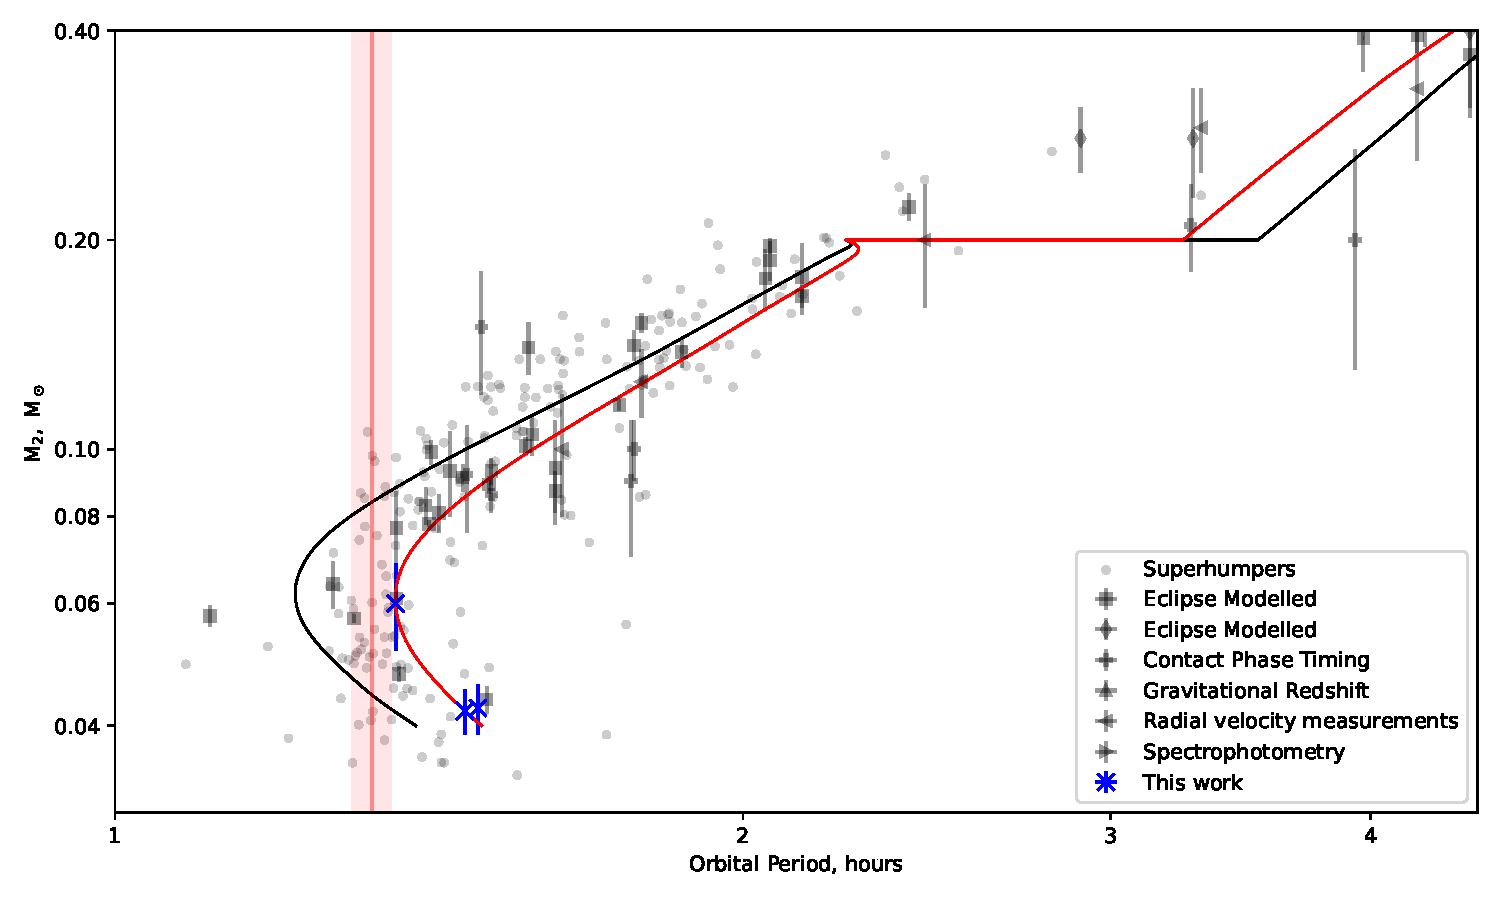
\includegraphics[width=\textwidth]{figures/results/three_cvs_with_weird_colours/GeneralFigs/M2_vs_P_withhumpers.pdf}
    \caption{Donor evolution tracks, from MESA, compared with observations. The observational sample presented here is the same as in \citet{wild2021}.}
    \label{fig:M2_vs_P}
\end{figure*}

\subsection{Is it correct to assume an unobscured white dwarf?}
\label{sect:impure white dwarf discussion}

As discussed in \S\ref{sect:three white dwarfs:method WD atmosphere fits}, the white dwarf colours may differ from model grids because the white dwarf ingress/egress is contaminated by an additional source of light, such as a boundary layer close to the surface.
If the eclipse is polluted by some other feature, phase-folded eclipse modelling will be wrong in two key elements: comparing colours to model atmospheres will be inaccurate, and the ingress and egress durations that constrain the white dwarf radius will not be correct.
\citet{Spark2015} conducted a study into the validity of assuming a pure white dwarf, comparing CV eclipse observations with white dwarfs with and without a few types of surface features such as boundary layers on the white dwarf, hot spots, or an optically thick or thin equatorial belt.
These features are revealed by a departure from symmetry between the white dwarf ingress and egress, but care must be taken not to confuse the flickering component of the CV with the signature of surface features.

Unfortunately, detecting a surface layer or hot spot on the white dwarf requires both a high time resolution and high signal-to-noise ratios. \citet{Spark2015} make use of SALTICAM data at a cadence of 0.15s, but the observations available here have a $\sim$3-4s exposure time and lower signal-to-noise. Measuring the eclipse precisely enough to make claims about the nature of the white dwarf's surface is therefore not possible with present observations.
The three systems of this work are prime candidates to search for WD eclipse asymmetries, as the issue of flickering corrupting the white dwarf ingress/egress derivative is largely mitigated; all three have little to no flickering present.
Future observations at higher cadence would open the possibility of examining the surfaces of these white dwarfs, though a large telescope will necessary due to the faintness of the systems; HiPERCAM on the GTC is an ideal candidate.


\subsection{The hot white dwarf of SSSJ0522-3505}
\label{sect:SSSJ0522-3505 white dwarf temperature discussion}

The effective temperature of white dwarfs in short period CVs is typically $\sim10000$K \citep{Pala2017a}, but the observed colours of SSSJ0522-3505 indicate a much hotter $T_{\rm eff}$ of $\sim25000$K. This is likely to be accurate, as the system's observations are clearly dominated by the white dwarf flux, and show roughly the same eclipse depth in the $r', g'$, and $u'$ bands, which would not be consistent with a lower white dwarf temperature.

The measured effective temperature could be wrong, either as a result of poor flux calibration (see \S\ref{sect:observations:flux calibrating the lightcurve} for reasons this is unlikely) or because the ingress/egress fluxes do not represent the fluxes of the white dwarf photosphere, as discussed in section~\ref{sect:impure white dwarf discussion}. However, the measured temperature is  $\sim10000$\,K hotter than expected, and these effects are unlikely to have introduced an error of this magnitude. As support for this, note that \citet{Pala2017a} find that white dwarf temperatures from UV spectroscopy typically agree with those measured from eclipse lightcurves to within $\sim1000$\,K. Reasons why the white dwarf temperature in SSSJ0522-3505 might be unusually hot are explored here, but UV spectroscopy to confirm the white dwarf temperature is highly desirable.

The white dwarf in a CV is thought to settle at an equilibrium temperature, where radiative heat loss is balanced with two energy sources: energy released by infalling material, and a low level of "simmering" nuclear fusion in the white dwarf envelope \citep{Townsley2003, Townsley2004}, but there are several reasons that this white dwarf may be temporarily out of equilibrium.
There is no reason, though it is unlikely, that a CV cannot form from a main sequence star with a brown dwarf companion, to produce a young CV with a low-mass donor and a white dwarf still cooling from its formation temperature.
Once the donor has reconnected with its Roche lobe, it would rejoin the normal CV evolution track and otherwise behave as a normal CV, with a normal accretion rate but a younger, hotter white dwarf than is typical.

A recent dwarf nova outburst was observed in this system in 2011, and could have produced a temporary boost to $T_{\rm eff}$. During these events, the disc enters a hot, optically thick state, and the infall rate onto the white dwarf is greatly increased \citep{osaki1996}, releasing a significant amount of energy and heating the white dwarf surface.
This is only the most recent \textit{observed} outburst, as there is a gap in observations between 2013 and 2019 during which any outburst events would have gone unrecorded. This may be important, as recent X-ray observations of another post period minimum system, OV Bootis \citep{Schwope2021}, shows that the WD temperature is increased to 23000K 5 months after outburst, 9000K hotter than its $T_{\rm eff}$ prior to outburst. The increase in temperature can be somewhat long-lasting; detailed observations of GW Lib have shown its WD is still 3000K hotter than equilibrium 8 years post-outburst\citep{Szkody2016}.
Another possibility is a recent classical nova -- thermonuclear runaway in an accreted surface layer on the white dwarf -- which would temporarily heat the white dwarf beyond its equilibrium temperature \citep{starrfield2016}, giving the impression of a hotter white dwarf than expected, though a classical nova resulting in such a strong heating effect would be surprising.

However, assuming the white dwarf is in thermal equilibrium, $T_{\rm eff}$ can be used to estimate the long-term accretion rate of the system \citep{townsley2009}.
If the modelled $T_{\rm eff}$ of SSSJ0522-3505 is both accurate and driven by accretion, it would correspond to $\dot M_{\rm WD} = 6\pm2 \times 10^{-10} M_\odot {\rm yr^{-1}}$, compared to accretion rates of $\sim10^{-10}-10^{-11} M_\odot {\rm yr^{-1}}$ expected for CVs in the post-period minimum regime \citep{Pala2017a}. Unfortunately, the MESA-based method to find $\dot M$ that is outlined in \S\ref{sect:modelling:evolutionary modelling} cannot be reliably applied to this system, as the $M_{\rm donor}$ is too low.
Whilst somewhat high, a mass accretion rate of $10^{-10} M_\odot {\rm yr^{-1}}$ is not incompatible with the presence of dwarf nova outbursts in SSSJ0522-3505, since a hot, optically thick accretion disc that would forbid such outbursts would require an accretion rate of order $10^{-8} M_\odot {\rm yr^{-1}}$ \citep{Hameury1998} to be stable on long timescales.
